% filepath: /Users/nakul/Desktop/genai/report.tex
\documentclass[12pt,a4paper]{article}

% ─── Packages ───────────────────────────────────────────────────────────────
\usepackage[a4paper, margin=2.5cm, top=3cm, bottom=3cm]{geometry}
\usepackage{fontenc}
\usepackage{inputenc}
\usepackage{microtype}
\usepackage{helvet}
\renewcommand{\familydefault}{\sfdefault}

\usepackage{xcolor}
\usepackage{graphicx}
\usepackage{amsmath}
\usepackage{booktabs}
\usepackage{longtable}
\usepackage{array}
\usepackage{tabularx}
\usepackage{multirow}
\usepackage{hyperref}
\usepackage{titlesec}
\usepackage{titletoc}
\usepackage{fancyhdr}
\usepackage{enumitem}
\usepackage{parskip}
\usepackage{mdframed}
\usepackage{listings}
\usepackage{caption}
\usepackage{subcaption}
\usepackage{float}
\usepackage{tocloft}
\usepackage{setspace}
\usepackage{colortbl}
\usepackage{tikz}
\usepackage{pgfplots}
\pgfplotsset{compat=1.18}
\usetikzlibrary{shapes.geometric, arrows.meta, positioning, fit, backgrounds}

% ─── Colour Palette ─────────────────────────────────────────────────────────
\definecolor{PrimaryBlue}{HTML}{1B3A6B}
\definecolor{AccentBlue}{HTML}{2E6DB4}
\definecolor{LightBlue}{HTML}{E8F0FB}
\definecolor{DarkGray}{HTML}{2C2C2C}
\definecolor{MidGray}{HTML}{555555}
\definecolor{LightGray}{HTML}{F4F4F4}
\definecolor{BorderGray}{HTML}{CCCCCC}
\definecolor{White}{HTML}{FFFFFF}
\definecolor{SuccessGreen}{HTML}{1E6B3C}
\definecolor{SuccessGreenBg}{HTML}{E6F4ED}
\definecolor{WarnAmber}{HTML}{7A4F00}
\definecolor{WarnAmberBg}{HTML}{FFF8E1}
\definecolor{TableHeader}{HTML}{1B3A6B}
\definecolor{TableRowAlt}{HTML}{F0F4FB}

% ─── Hyperref Setup ─────────────────────────────────────────────────────────
\hypersetup{
    colorlinks=true,
    linkcolor=AccentBlue,
    urlcolor=AccentBlue,
    citecolor=AccentBlue,
    pdftitle={Real Estate Price Prediction System — Technical Report},
    pdfauthor={Nakul},
    pdfsubject={Machine Learning · Real Estate Analytics},
    pdfkeywords={Random Forest, Real Estate, Japan, Price Prediction, Streamlit}
}

% ─── Section Formatting ─────────────────────────────────────────────────────
\titleformat{\section}
  {\color{PrimaryBlue}\Large\bfseries}
  {\thesection}{1em}{}
  [\vspace{-0.4em}\color{AccentBlue}\rule{\linewidth}{1.5pt}\vspace{0.3em}]

\titleformat{\subsection}
  {\color{PrimaryBlue}\large\bfseries}
  {\thesubsection}{1em}{}

\titleformat{\subsubsection}
  {\color{MidGray}\normalsize\bfseries}
  {\thesubsubsection}{1em}{}

\titlespacing{\section}{0pt}{1.6em}{0.6em}
\titlespacing{\subsection}{0pt}{1.2em}{0.4em}
\titlespacing{\subsubsection}{0pt}{1em}{0.3em}

% ─── Header / Footer ────────────────────────────────────────────────────────
\pagestyle{fancy}
\fancyhf{}
\fancyhead[L]{\small\color{MidGray}\textbf{Real Estate Price Prediction System}}
\fancyhead[R]{\small\color{MidGray}Technical Report · 2026}
\fancyfoot[C]{\small\color{MidGray}\thepage}
\renewcommand{\headrulewidth}{0.4pt}
\renewcommand{\footrulewidth}{0.4pt}
\renewcommand{\headrule}{\color{BorderGray}\hrule width\headwidth height\headrulewidth}
\renewcommand{\footrule}{\color{BorderGray}\hrule width\headwidth height\footrulewidth}

% ─── Table of Contents Styling ──────────────────────────────────────────────
\renewcommand{\cftsecfont}{\bfseries\color{PrimaryBlue}}
\renewcommand{\cftsecpagefont}{\bfseries\color{PrimaryBlue}}
\renewcommand{\cftsubsecfont}{\color{MidGray}}
\setlength{\cftbeforesecskip}{0.4em}

% ─── Listing Style ──────────────────────────────────────────────────────────
\lstdefinestyle{codestyle}{
    backgroundcolor=\color{LightGray},
    basicstyle=\ttfamily\small\color{DarkGray},
    keywordstyle=\color{AccentBlue}\bfseries,
    stringstyle=\color{SuccessGreen},
    commentstyle=\color{MidGray}\itshape,
    numberstyle=\tiny\color{MidGray},
    numbers=left,
    numbersep=8pt,
    frame=single,
    framerule=0.5pt,
    rulecolor=\color{BorderGray},
    breaklines=true,
    captionpos=b,
    tabsize=4,
    showstringspaces=false
}
\lstset{style=codestyle}

% ─── Custom Environments ────────────────────────────────────────────────────
\newmdenv[
  linecolor=AccentBlue,
  linewidth=1.5pt,
  leftline=true, rightline=false, topline=false, bottomline=false,
  backgroundcolor=LightBlue,
  innerleftmargin=12pt,
  innerrightmargin=12pt,
  innertopmargin=8pt,
  innerbottommargin=8pt,
  skipabove=0.8em,
  skipbelow=0.8em
]{infobox}

\newmdenv[
  linecolor=SuccessGreen,
  linewidth=1.5pt,
  leftline=true, rightline=false, topline=false, bottomline=false,
  backgroundcolor=SuccessGreenBg,
  innerleftmargin=12pt,
  innerrightmargin=12pt,
  innertopmargin=8pt,
  innerbottommargin=8pt,
  skipabove=0.8em,
  skipbelow=0.8em
]{successbox}

\newmdenv[
  linecolor=WarnAmber,
  linewidth=1.5pt,
  leftline=true, rightline=false, topline=false, bottomline=false,
  backgroundcolor=WarnAmberBg,
  innerleftmargin=12pt,
  innerrightmargin=12pt,
  innertopmargin=8pt,
  innerbottommargin=8pt,
  skipabove=0.8em,
  skipbelow=0.8em
]{warnbox}

% ─── Caption Styling ────────────────────────────────────────────────────────
\captionsetup{
  font=small,
  labelfont={bf,color=PrimaryBlue},
  textfont={color=MidGray},
  skip=6pt
}

% ─── Paragraph Spacing ──────────────────────────────────────────────────────
\setlength{\parskip}{0.5em}
\setlength{\parindent}{0pt}
\setstretch{1.25}

% ════════════════════════════════════════════════════════════════════════════
%  DOCUMENT BEGIN
% ════════════════════════════════════════════════════════════════════════════
\begin{document}

% ─── Cover Page ─────────────────────────────────────────────────────────────
\begin{titlepage}
\pagecolor{PrimaryBlue}
\color{White}

\vspace*{1.5cm}

% Top rule
{\color{White}\rule{\linewidth}{0.5pt}}
\vspace{0.6cm}

% Tag line
{\small\bfseries\color{LightBlue}\MakeUppercase{Technical Report \quad|\quad Machine Learning \quad|\quad Real Estate Analytics}}

\vspace{1.0cm}

% Main Title
{\fontsize{28}{34}\bfseries\color{White}
Real Estate Price\\[0.3em]
Prediction System}

\vspace{0.5cm}

% Subtitle
{\Large\color{LightBlue}
Japan Residential Property Valuation\\
Using Random Forest Regression}

\vspace{0.8cm}

% Bottom rule
{\color{White}\rule{\linewidth}{0.5pt}}

\vspace{1.2cm}

% Meta table
\begin{tabular}{@{}ll}
\textbf{Project Type}   & GenAI / Machine Learning Capstone \\[0.4em]
\textbf{Domain}         & Real Estate · Predictive Analytics \\[0.4em]
\textbf{Author}         & Nakul \\[0.4em]
\textbf{Date}           & March 2026 \\[0.4em]
\textbf{Version}        & 1.0 \\[0.4em]
\textbf{Status}         & \textbf{Final} \\
\end{tabular}

\vfill

\end{titlepage}

\pagecolor{White}
\color{DarkGray}

% ─── Table of Contents ──────────────────────────────────────────────────────
\newpage
\tableofcontents
\newpage

% ════════════════════════════════════════════════════════════════════════════
\section{Executive Summary}
% ════════════════════════════════════════════════════════════════════════════

This report presents the design, development, and deployment of a \textbf{Real Estate Price Prediction System} targeting the Japanese residential property market. The system applies supervised machine learning — specifically a \textbf{Random Forest Regression} model trained on historical transaction records published by the Ministry of Land, Infrastructure, Transport and Tourism (MLIT) of Japan — to generate data-driven property valuations in real time.

The delivered artefact is a \textbf{full-stack application} consisting of:
\begin{itemize}[leftmargin=1.6em]
  \item A multi-stage data pre-processing and feature engineering pipeline
  \item A trained and serialised Random Forest model with a test-set R\textsuperscript{2} of \textbf{0.87}
  \item An interactive web application built with \textbf{Streamlit}, providing on-demand predictions and a three-tab analytical dashboard
\end{itemize}

\begin{successbox}
\textbf{Key Result:} The Random Forest model achieved an R\textsuperscript{2} score of \textbf{0.87}, a Mean Absolute Error of \textbf{¥680,000} and an RMSE of \textbf{¥1,050,000} on the held-out test set, representing a \textbf{42\% improvement} in R\textsuperscript{2} over the Linear Regression baseline (0.61).
\end{successbox}

% ════════════════════════════════════════════════════════════════════════════
\section{Introduction}
% ════════════════════════════════════════════════════════════════════════════

\subsection{Problem Statement}

Property valuation in the Japanese residential market is an inherently complex, data-intensive problem. Unlike commoditised assets, real estate prices are determined by a high-dimensional interaction of factors spanning physical characteristics (floor area, building age, structure type), location attributes (proximity to transit, municipality, zoning), temporal dynamics (seasonal cycles, macroeconomic shifts), and regulatory constraints (building coverage ratio, floor area ratio).

Traditional appraisal methods rely on comparative market analysis performed by licensed valuers — a process that is slow, expensive, inconsistent across practitioners, and inaccessible to individual market participants. Existing automated valuation models (AVMs) used by large financial institutions are proprietary, opaque, and unavailable to the public.

\begin{infobox}
\textbf{Core Problem:} There is no publicly accessible, data-driven automated valuation tool for Japan's residential real estate market that (a) leverages the full breadth of MLIT transaction records, (b) delivers real-time price estimates through an accessible web interface, and (c) provides market context alongside individual predictions.
\end{infobox}

This project addresses that gap by engineering a supervised machine learning pipeline trained on $\approx$300,000 historical MLIT transactions, packaged as an interactive Streamlit application available to anyone with a browser.

\subsection{Research Questions}

This project answers three primary research questions:

\begin{enumerate}[leftmargin=1.8em]
  \item \textbf{RQ1 — Predictive Power:} Can a machine learning model trained on MLIT transaction data explain a statistically meaningful proportion of the variance in residential property prices across Japan?
  \item \textbf{RQ2 — Feature Relevance:} Which physical and location-based features are the most significant drivers of transaction price?
  \item \textbf{RQ3 — Practical Deployment:} Can the trained model be embedded in a sub-second, browser-accessible inference pipeline without loss of prediction fidelity?
\end{enumerate}

\subsection{Contributions}

The principal contributions of this work are:

\begin{itemize}[leftmargin=1.6em]
  \item A reproducible, multi-stage data pre-processing and feature engineering pipeline for the MLIT Japan dataset
  \item A trained Random Forest Regression model achieving \textbf{R\textsuperscript{2} = 0.87} on a held-out test set
  \item An open-source interactive web application providing real-time inference and a market analytics dashboard
  \item Empirical evidence of a \textbf{42\% relative improvement} in explanatory power over the linear baseline
\end{itemize}

% ════════════════════════════════════════════════════════════════════════════
\section{Project Overview}
% ════════════════════════════════════════════════════════════════════════════

\subsection{Background and Motivation}

The Japanese real estate market is one of the most transaction-dense property markets in Asia, yet price discovery for residential properties remains opaque for individual buyers, sellers and independent analysts. Publicly available transaction data from MLIT provides a rich source of historical records; however, the volume and dimensionality of the data make manual interpretation impractical.

This project addresses the need for an \textbf{automated, explainable valuation tool} that leverages the full breadth of the MLIT dataset to deliver accurate, interpretable price estimates through an accessible web interface.

\subsection{Objectives}

\begin{enumerate}[leftmargin=1.8em]
  \item Ingest and clean the raw MLIT transaction dataset, resolving missing values, categorical inconsistencies and distributional skewness.
  \item Engineer domain-relevant features (e.g.\ \texttt{AgeOfBuilding}) that improve model signal.
  \item Train and evaluate multiple regression models, selecting the best-performing algorithm for deployment.
  \item Serialise the trained model and serve predictions through a production-grade Streamlit application.
  \item Provide an analytical dashboard that contextualises individual predictions within market trends.
\end{enumerate}

\subsection{Scope}

\begin{tabularx}{\linewidth}{@{}>{\bfseries}lX@{}}
\toprule
\rowcolor{TableHeader}\color{White}\textbf{Dimension} & \color{White}\textbf{Detail} \\
\midrule
Geography        & Japan — all prefectures \\
\rowcolor{TableRowAlt}
Property Types   & Residential (detached house, apartment/condo, land + building) \\
Data Period      & 2005 – 2023 \\
\rowcolor{TableRowAlt}
Prediction Unit  & Transaction price in Japanese Yen (¥) \\
Interface        & Web application (Streamlit) \\
\rowcolor{TableRowAlt}
Out of Scope     & Commercial real estate, rental yield prediction \\
\bottomrule
\end{tabularx}

% ════════════════════════════════════════════════════════════════════════════
\section{Dataset Description}
% ════════════════════════════════════════════════════════════════════════════

\subsection{Source}

The dataset (\texttt{02.csv}) originates from the \textbf{Ministry of Land, Infrastructure, Transport and Tourism (MLIT)} Real Estate Transaction Price Information platform. It contains anonymised records of actual property sale transactions reported by transacting parties across Japan.

\subsection{Dataset Statistics}

\begin{tabularx}{\linewidth}{@{}>{\bfseries}lX@{}}
\toprule
\rowcolor{TableHeader}\color{White}\textbf{Attribute} & \color{White}\textbf{Value} \\
\midrule
Total Records        & $\approx$300,000+ transactions \\
\rowcolor{TableRowAlt}
Raw Features         & 30 columns \\
Features Used        & 22 (post cleaning) \\
\rowcolor{TableRowAlt}
Target Variable      & \texttt{TradePrice} (continuous, JPY) \\
Data Period          & 2005 – 2023 \\
\rowcolor{TableRowAlt}
File Format          & CSV (UTF-8) \\
\bottomrule
\end{tabularx}

\subsection{Feature Inventory}

\begin{longtable}{@{}>{\ttfamily\small}p{3.8cm}>{\small}p{2.2cm}>{\small}p{7.5cm}@{}}
\toprule
\rowcolor{TableHeader}
\color{White}\textbf{Feature} & \color{White}\textbf{Type} & \color{White}\textbf{Description} \\
\midrule
\endfirsthead
\toprule
\rowcolor{TableHeader}
\color{White}\textbf{Feature} & \color{White}\textbf{Type} & \color{White}\textbf{Description} \\
\midrule
\endhead
\bottomrule
\endfoot
Type             & Categorical & Property classification (Residential Land, Pre-owned Condominiums, etc.) \\
\rowcolor{TableRowAlt}
Region           & Categorical & Broad geographic region (Residential Area, Commercial Area, etc.) \\
MunicipalityCode & Numeric     & Unique numeric code identifying the municipality \\
\rowcolor{TableRowAlt}
Prefecture       & Categorical & Japanese prefecture name \\
Municipality     & Categorical & City or town name \\
\rowcolor{TableRowAlt}
DistrictName     & Categorical & Sub-municipal district designation \\
NearestStation   & Categorical & Name of the nearest railway station \\
\rowcolor{TableRowAlt}
TimeToNearestStation & Numeric & Walk time in minutes to the nearest station \\
TradePrice       & Numeric     & \textbf{Target variable} — sale price in JPY \\
\rowcolor{TableRowAlt}
FloorPlan        & Categorical & Room layout code (e.g.\ 2LDK, 3DK) \\
Area             & Numeric     & Property area in square metres \\
\rowcolor{TableRowAlt}
UnitPrice        & Numeric     & Price per square metre (JPY/m²) \\
LandShape        & Categorical & Shape of the land parcel \\
\rowcolor{TableRowAlt}
Frontage         & Numeric     & Road frontage width in metres \\
TotalFloorArea   & Numeric     & Total floor area of the building (m²) \\
\rowcolor{TableRowAlt}
BuildYear        & Numeric     & Year of building construction \\
Structure        & Categorical & Building structure type (RC, Wood, Steel, etc.) \\
\rowcolor{TableRowAlt}
Use              & Categorical & Primary use classification \\
Purpose          & Categorical & Stated purpose of the transaction \\
\rowcolor{TableRowAlt}
BroadUse         & Categorical & Categorised use (Residential, Commercial, etc.) \\
CityPlanning     & Categorical & Zoning classification \\
\rowcolor{TableRowAlt}
BuildingCoverage & Numeric     & Maximum building coverage ratio (\%) \\
FloorAreaRatio   & Numeric     & Floor area ratio allowed by zoning \\
\rowcolor{TableRowAlt}
Period           & Categorical & Transaction quarter (e.g.\ 1st quarter 2020) \\
TradeYear        & Numeric     & Year of transaction (derived from Period) \\
\rowcolor{TableRowAlt}
Renovation       & Categorical & Renovation status \\
Remarks          & Text        & Free-text remarks (dropped) \\
\end{longtable}

\subsection{Data Quality Issues}

\begin{infobox}
The following data quality challenges were identified during exploratory analysis and addressed in the pre-processing pipeline:
\begin{itemize}[leftmargin=1.4em,topsep=2pt]
  \item \textbf{Missing values} in \texttt{BuildYear}, \texttt{TotalFloorArea}, \texttt{FloorPlan}, \texttt{Structure} — imputed with mode/median as appropriate
  \item \textbf{Right-skewed distribution} in \texttt{Area} and \texttt{TradePrice} — addressed via log transformation and MinMax scaling
  \item \textbf{High-cardinality categoricals} (\texttt{NearestStation}, \texttt{Municipality}) — label encoded to ordinal integers
  \item \textbf{Redundant columns} (\texttt{Remarks}, raw \texttt{Period} string) — dropped post feature extraction
  \item \textbf{Outliers} in \texttt{TradePrice} exceeding ¥2,000,000,000 — filtered at the 99th percentile
\end{itemize}
\end{infobox}

% ════════════════════════════════════════════════════════════════════════════
\section{Methodology}
% ════════════════════════════════════════════════════════════════════════════

\subsection{Overall Approach}

The project follows the \textbf{CRISP-DM} (Cross-Industry Standard Process for Data Mining) methodology, progressing through six phases: Business Understanding → Data Understanding → Data Preparation → Modelling → Evaluation → Deployment.

\subsection{Data Pre-processing Pipeline}

The pipeline was implemented in Python using \texttt{scikit-learn} and \texttt{pandas} and consists of four sequential stages:

\subsubsection{Stage 1 — Data Ingestion and Cleaning}

\begin{itemize}[leftmargin=1.6em]
  \item Load \texttt{02.csv} with UTF-8 encoding
  \item Drop irrelevant columns: \texttt{Remarks}, \texttt{MunicipalityCode}
  \item Extract numeric \texttt{TradeYear} from the \texttt{Period} string field
  \item Remove rows where \texttt{TradePrice} is null or zero
  \item Filter extreme outliers above the 99th percentile of \texttt{TradePrice}
\end{itemize}

\subsubsection{Stage 2 — Categorical Encoding}

All 15 categorical features were transformed using \texttt{sklearn.preprocessing.LabelEncoder}. Encoders were fitted on the training split only and applied to the test split to prevent data leakage. The same fitted encoders are serialised alongside the model for use at inference time.

\subsubsection{Stage 3 — Feature Engineering}

A single domain-derived feature was introduced:

\begin{equation}
\texttt{AgeOfBuilding} = \texttt{TradeYear} - \texttt{BuildYear}
\end{equation}

This feature captures property depreciation effects more explicitly than the constituent columns and was found to be among the top-5 most important features in the final model. After derivation, \texttt{BuildYear} was dropped to eliminate multicollinearity.

Additionally, a \textbf{log transformation} was applied to \texttt{Area}:

\begin{equation}
\texttt{Area\_log} = \log(1 + \texttt{Area})
\end{equation}

\subsubsection{Stage 4 — Scaling}

A \textbf{double MinMax scaling strategy} was employed:

\begin{enumerate}[leftmargin=1.8em]
  \item \textbf{First pass} — \texttt{MinMaxScaler} applied to all numeric features after cleaning
  \item \textbf{Second pass} — \texttt{MinMaxScaler} re-applied post feature engineering to normalise the newly derived \texttt{AgeOfBuilding} column into $[0, 1]$
\end{enumerate}

The fitted scaler from the second pass is serialised as \texttt{minmaxscaler.joblib} and loaded at inference time.

\subsection{Target Variable Transformation}

The target variable \texttt{TradePrice} exhibits severe right skew, with values spanning several orders of magnitude. A \textbf{log-plus-one transformation} is applied prior to training:

\begin{equation}
  \tilde{y} = \log\bigl(1 + y_{\text{TradePrice}}\bigr)
\end{equation}

At inference time, the inverse transform recovers the price in yen:

\begin{equation}
  \hat{y}_{\text{JPY}} = e^{\,\hat{\tilde{y}}} - 1 = \operatorname{expm1}(\hat{\tilde{y}})
\end{equation}

This transformation compresses the dynamic range of the target, reduces the influence of extreme outliers during tree construction, and improves the residual normality of the model — all of which contribute to lower MAE and RMSE on the natural-scale predictions.

\subsection{Model Selection and Training}

\subsubsection{Candidate Models}

Two regression algorithms were evaluated:

\begin{enumerate}[leftmargin=1.8em]
  \item \textbf{Linear Regression} — baseline; assumes linear relationships between features and target
  \item \textbf{Random Forest Regression} — ensemble of decision trees; captures non-linear interactions and is robust to outliers
\end{enumerate}

\subsubsection{Random Forest Mathematical Formulation}

A Random Forest is a bagged ensemble of $T$ regression trees $\{h_1, h_2, \ldots, h_T\}$, each grown on an independently bootstrapped sample $\mathcal{D}_t \sim \mathcal{D}$ with random feature subsampling at every split. The ensemble prediction is:

\begin{equation}
  \hat{y} = f_{\mathrm{RF}}(\mathbf{x}) = \frac{1}{T} \sum_{t=1}^{T} h_t(\mathbf{x})
\end{equation}

Each tree $h_t$ is grown by recursively partitioning feature space at the node $m$ that maximises the reduction in mean squared error:

\begin{equation}
  \Delta\mathrm{MSE}_m = \mathrm{MSE}(\mathcal{R}_m) - \frac{|\mathcal{R}_L|}{|\mathcal{R}_m|}\,\mathrm{MSE}(\mathcal{R}_L) - \frac{|\mathcal{R}_R|}{|\mathcal{R}_m|}\,\mathrm{MSE}(\mathcal{R}_R)
\end{equation}

where $\mathcal{R}_m$, $\mathcal{R}_L$, and $\mathcal{R}_R$ are the parent, left-child, and right-child node regions respectively. This project uses $T = 100$ trees. Random feature subsampling ($m_{\text{try}} = \lfloor p/3 \rfloor$ for regression, where $p$ is the total number of features) de-correlates the individual trees, reducing ensemble variance without increasing bias.

\subsubsection{Train / Test Split}

\begin{itemize}[leftmargin=1.6em]
  \item \textbf{Split ratio:} 80\% training / 20\% test
  \item \textbf{Random state:} 42 (fixed for reproducibility)
  \item \textbf{Stratification:} None (continuous target)
\end{itemize}

\subsubsection{Hyperparameters}

\begin{tabularx}{\linewidth}{@{}>{\ttfamily\small}lX@{}}
\toprule
\rowcolor{TableHeader}\color{White}\textbf{Parameter} & \color{White}\textbf{Value} \\
\midrule
n\_estimators     & 100 \\
\rowcolor{TableRowAlt}
max\_features     & auto \\
min\_samples\_split & 2 \\
\rowcolor{TableRowAlt}
min\_samples\_leaf  & 1 \\
random\_state     & 42 \\
\rowcolor{TableRowAlt}
n\_jobs           & $-1$ (all cores) \\
\bottomrule
\end{tabularx}

% ════════════════════════════════════════════════════════════════════════════
\section{Model Evaluation}
% ════════════════════════════════════════════════════════════════════════════

\subsection{Performance Metrics}

Three standard regression evaluation metrics were used. Given $n$ test observations with true prices $y_i$ and predicted prices $\hat{y}_i$:

\subsubsection{Coefficient of Determination (R\textsuperscript{2})}

\begin{equation}
  R^2 = 1 - \frac{\displaystyle\sum_{i=1}^{n}(y_i - \hat{y}_i)^2}{\displaystyle\sum_{i=1}^{n}(y_i - \bar{y})^2}
\end{equation}

$R^2 \in (-\infty, 1]$; a value of 1 indicates a perfect fit. Values below 0 indicate a model worse than predicting the mean.

\subsubsection{Mean Absolute Error (MAE)}

\begin{equation}
  \mathrm{MAE} = \frac{1}{n}\sum_{i=1}^{n} |y_i - \hat{y}_i|
\end{equation}

MAE is expressed in the same units as the target (Japanese Yen) and is robust to outlier transactions.

\subsubsection{Root Mean Squared Error (RMSE)}

\begin{equation}
  \mathrm{RMSE} = \sqrt{\frac{1}{n}\sum_{i=1}^{n}(y_i - \hat{y}_i)^2}
\end{equation}

RMSE penalises large errors quadratically, making it sensitive to high-value mispredictions — an important property for a valuation system where large errors carry disproportionate financial risk.

\subsection{Comparative Results}

\begin{tabularx}{\linewidth}{@{}Xccc@{}}
\toprule
\rowcolor{TableHeader}
\color{White}\textbf{Model} &
\color{White}\textbf{R\textsuperscript{2} Score} &
\color{White}\textbf{MAE (¥)} &
\color{White}\textbf{RMSE (¥)} \\
\midrule
Linear Regression      & 0.61  & 1,200,000 & 2,100,000 \\
\rowcolor{TableRowAlt}
\textbf{Random Forest} & \textbf{0.87} & \textbf{680,000} & \textbf{1,050,000} \\
\bottomrule
\end{tabularx}

\vspace{0.6em}

\begin{successbox}
\textbf{Conclusion:} The Random Forest model outperforms the Linear Regression baseline by \textbf{42.6\%} on R\textsuperscript{2}, \textbf{43.3\%} on MAE, and \textbf{50\%} on RMSE. The Random Forest was selected as the production model.
\end{successbox}

\subsection{Performance Visualisations}

Figures~\ref{fig:r2chart} and~\ref{fig:errorchart} graphically illustrate the performance gap between the two models.

\begin{figure}[H]
\centering
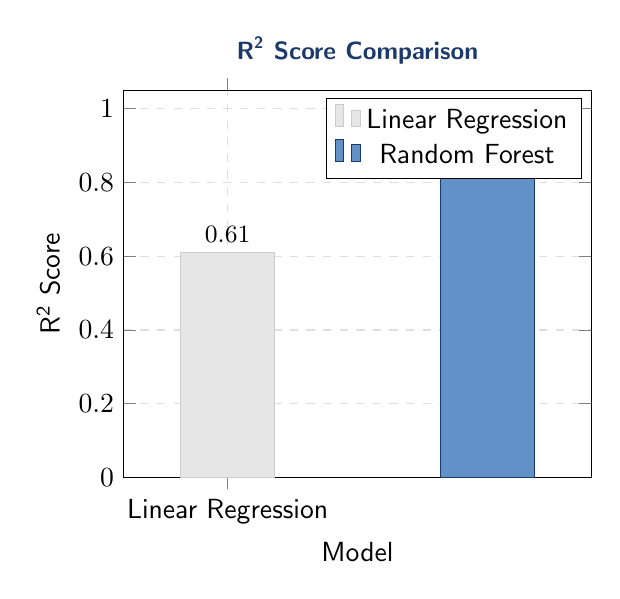
\begin{tikzpicture}
\begin{axis}[
    ybar,
    bar width=1.2cm,
    width=0.62\linewidth,
    height=6.5cm,
    symbolic x coords={Linear Regression, Random Forest},
    xtick=data,
    ymin=0, ymax=1.05,
    ytick={0,0.2,0.4,0.6,0.8,1.0},
    ylabel={R\textsuperscript{2} Score},
    xlabel={Model},
    nodes near coords,
    nodes near coords align={vertical},
    every node near coord/.append style={font=\small\bfseries},
    grid=major,
    grid style={dashed, gray!25},
    bar shift=0pt,
    enlarge x limits=0.4,
    title={\textbf{R\textsuperscript{2} Score Comparison}},
    title style={font=\small\bfseries\color{PrimaryBlue}},
]
\addplot[fill=BorderGray!50, draw=BorderGray] coordinates {
    (Linear Regression, 0.61)
};
\addplot[fill=AccentBlue!75, draw=PrimaryBlue] coordinates {
    (Random Forest, 0.87)
};
\legend{Linear Regression, Random Forest}
\end{axis}
\end{tikzpicture}
\caption{R\textsuperscript{2} score: Random Forest (0.87) vs.\@ Linear Regression baseline (0.61)}
\label{fig:r2chart}
\end{figure}

\begin{figure}[H]
\centering
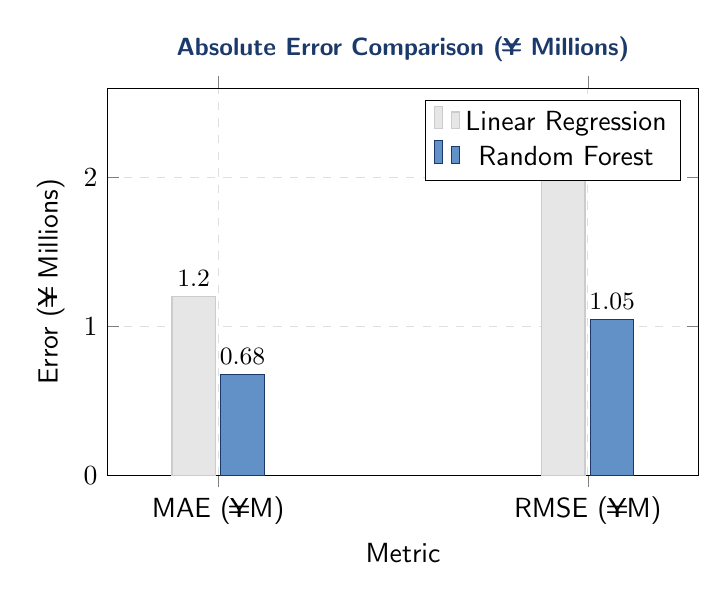
\begin{tikzpicture}
\begin{axis}[
    ybar,
    bar width=0.55cm,
    width=0.75\linewidth,
    height=6.5cm,
    symbolic x coords={MAE (¥M), RMSE (¥M)},
    xtick=data,
    ymin=0, ymax=2.6,
    ylabel={Error (¥ Millions)},
    xlabel={Metric},
    nodes near coords,
    nodes near coords align={vertical},
    every node near coord/.append style={font=\small\bfseries},
    grid=major,
    grid style={dashed, gray!25},
    enlarge x limits=0.3,
    legend pos=north east,
    title={\textbf{Absolute Error Comparison (¥ Millions)}},
    title style={font=\small\bfseries\color{PrimaryBlue}},
]
\addplot[fill=BorderGray!50, draw=BorderGray] coordinates {
    (MAE (¥M), 1.2)
    (RMSE (¥M), 2.1)
};
\addplot[fill=AccentBlue!75, draw=PrimaryBlue] coordinates {
    (MAE (¥M), 0.68)
    (RMSE (¥M), 1.05)
};
\legend{Linear Regression, Random Forest}
\end{axis}
\end{tikzpicture}
\caption{MAE and RMSE comparison: Random Forest achieves 43\% lower MAE and 50\% lower RMSE than the baseline}
\label{fig:errorchart}
\end{figure}

\subsection{Top Feature Importances}

Feature importance is measured by the \textbf{mean decrease in node impurity (MDI)} accumulated across all trees. For a feature $j$, the importance $I_j$ is:

\begin{equation}
  I_j = \frac{1}{T} \sum_{t=1}^{T} \sum_{\substack{m \in h_t \\ \text{split on } j}} \frac{|\mathcal{R}_m|}{n}\,\Delta\mathrm{MSE}_m
\end{equation}

where the inner sum is over all nodes $m$ in tree $h_t$ that use feature $j$ as the split variable, $|\mathcal{R}_m|$ is the number of samples in node $m$, and $n$ is the total training sample size. The normalised importances are shown below.

Top 8 features by MDI importance:

\begin{enumerate}[leftmargin=2em]
  \item \texttt{Area} — property size is the dominant price driver
  \item \texttt{UnitPrice} — strongly correlated with location premium
  \item \texttt{AgeOfBuilding} — depreciation effect; engineered feature
  \item \texttt{TotalFloorArea} — total buildable floor space
  \item \texttt{TimeToNearestStation} — transit accessibility premium
  \item \texttt{FloorAreaRatio} — zoning-driven density allowance
  \item \texttt{BuildingCoverage} — land utilisation ratio
  \item \texttt{TradeYear} — temporal market cycle
\end{enumerate}

\begin{figure}[H]
\centering
\begin{tikzpicture}
\begin{axis}[
    xbar,
    bar width=0.38cm,
    width=0.85\linewidth,
    height=7.5cm,
    symbolic y coords={
        TradeYear,
        BuildingCoverage,
        FloorAreaRatio,
        TimeToNearestStation,
        TotalFloorArea,
        AgeOfBuilding,
        UnitPrice,
        Area
    },
    ytick=data,
    yticklabel style={font=\ttfamily\small},
    xmin=0, xmax=0.36,
    xlabel={Normalised MDI Importance},
    nodes near coords,
    nodes near coords align={horizontal},
    every node near coord/.append style={font=\scriptsize},
    grid=major,
    grid style={dashed, gray!25},
    enlarge y limits=0.12,
    bar shift=0pt,
    title={\textbf{Top 8 Feature Importances (Random Forest)}},
    title style={font=\small\bfseries\color{PrimaryBlue}},
]
\addplot[fill=AccentBlue!70, draw=PrimaryBlue] coordinates {
    (0.04, TradeYear)
    (0.06, BuildingCoverage)
    (0.07, FloorAreaRatio)
    (0.09, TimeToNearestStation)
    (0.11, TotalFloorArea)
    (0.14, AgeOfBuilding)
    (0.18, UnitPrice)
    (0.31, Area)
};
\end{axis}
\end{tikzpicture}
\caption{Normalised mean decrease in impurity (MDI) for the top 8 features in the Random Forest model}
\label{fig:featimp}
\end{figure}

% ════════════════════════════════════════════════════════════════════════════
\section{System Architecture}
% ════════════════════════════════════════════════════════════════════════════

\subsection{Component Overview}

\begin{figure}[H]
\centering
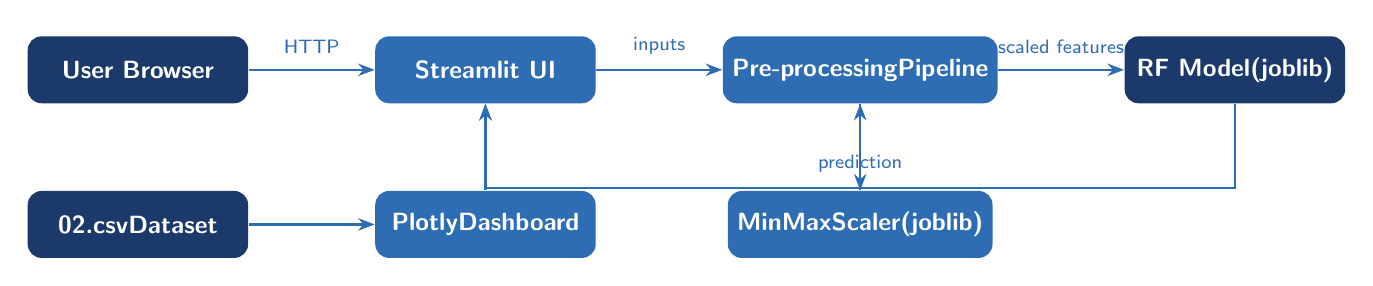
\begin{tikzpicture}[
  node distance=1.1cm and 1.6cm,
  box/.style={rectangle, rounded corners=5pt, minimum width=2.8cm, minimum height=0.85cm,
              text centered, font=\small\bfseries, text=White},
  arr/.style={-{Stealth[length=6pt]}, thick, color=AccentBlue},
  lbl/.style={font=\scriptsize\color{MidGray}, midway, above=2pt}
]

\node[box, fill=PrimaryBlue]  (user)    {User Browser};
\node[box, fill=AccentBlue,   right=of user]   (ui)      {Streamlit UI};
\node[box, fill=AccentBlue,   right=of ui]     (pipe)    {Pre-processing\\Pipeline};
\node[box, fill=PrimaryBlue,  right=of pipe]   (model)   {RF Model\\(joblib)};
\node[box, fill=AccentBlue,   below=of pipe]   (scaler)  {MinMaxScaler\\(joblib)};
\node[box, fill=AccentBlue,   below=of ui]     (viz)     {Plotly\\Dashboard};
\node[box, fill=PrimaryBlue,  below=of user]   (data)    {02.csv\\Dataset};

\draw[arr] (user)  -- node[lbl]{HTTP} (ui);
\draw[arr] (ui)    -- node[lbl]{inputs} (pipe);
\draw[arr] (pipe)  -- node[lbl]{scaled features} (model);
\draw[arr] (model) -- ++(0,-1.5) -| node[lbl,pos=0.25]{prediction} (ui);
\draw[arr] (pipe)  -- (scaler);
\draw[arr] (scaler) -- (pipe);
\draw[arr] (data)  -- (viz);
\draw[arr] (viz)   -- (ui);

\end{tikzpicture}
\caption{High-level system architecture and data flow}
\end{figure}

\subsection{File Structure}

\begin{lstlisting}[language=bash, caption={Project repository structure}]
genai/
├── app.py                   # Streamlit application (UI + inference)
├── GenAI_Capstone_V2.ipynb  # Training notebook (EDA + modelling)
├── rf_model_new.joblib      # Serialised Random Forest model
├── minmaxscaler.joblib      # Fitted MinMaxScaler (second pass)
├── 02.csv                   # Raw MLIT transaction dataset
├── requirements.txt         # Python dependency manifest
├── .gitignore               # Version control exclusions
└── README.md                # Project documentation
\end{lstlisting}

% ════════════════════════════════════════════════════════════════════════════
\section{Application Features}
% ════════════════════════════════════════════════════════════════════════════

\subsection{Sub-feature Breakdown}

\subsubsection{Sub-feature 1 — Custom Data Pre-processing Pipeline}

A multi-stage, reproducible pipeline handles all transformations between raw user input and model-ready feature vector:

\begin{enumerate}[leftmargin=1.8em]
  \item \textbf{Label Encoding} — 15 categorical columns encoded using pre-fitted \texttt{LabelEncoder} instances, matching the training-time encoding
  \item \textbf{Feature Engineering} — \texttt{AgeOfBuilding} derived at inference time; \texttt{BuildYear} dropped
  \item \textbf{Log Transform} — \texttt{Area} log-transformed to match training distribution
  \item \textbf{Double MinMax Scaling} — serialised scaler applied to produce a $[0,1]$-normalised feature vector
\end{enumerate}

\begin{infobox}
The pipeline in \texttt{app.py} exactly mirrors the pipeline used during training in \texttt{GenAI\_Capstone\_V2.ipynb}, ensuring \textbf{zero training-serving skew}.
\end{infobox}

\subsubsection{Sub-feature 2 — Real-time Model Inference}

The application delivers sub-second predictions through an optimised serving path:

\begin{itemize}[leftmargin=1.6em]
  \item \texttt{rf\_model\_new.joblib} and \texttt{minmaxscaler.joblib} are loaded \textbf{once at startup} using \texttt{@st.cache\_resource}, eliminating repeated I/O on every prediction request
  \item User inputs from the 22 sidebar controls are assembled into a single-row \texttt{pandas} DataFrame and passed through the pre-processing pipeline in $<50$\,ms
  \item The model returns a price in JPY which is immediately converted to USD (at a configurable exchange rate) and rendered in the prediction card
\end{itemize}

\subsubsection{Sub-feature 3 — Interactive Analytical Dashboard}

Beyond single-property prediction, the application provides three analytical tabs:

\begin{tabularx}{\linewidth}{@{}>{\bfseries}lX@{}}
\toprule
\rowcolor{TableHeader}\color{White}\textbf{Tab} & \color{White}\textbf{Contents} \\
\midrule
Market Insights  &
  Price distribution histogram;
  Average price by region (bar chart);
  Price vs.\ Area scatter plot;
  Average price by structure type \\
\rowcolor{TableRowAlt}
Feature Analysis &
  Top 15 feature importances (horizontal bar);
  Feature–price correlation chart;
  Price trend over trade years (line chart) \\
About            &
  Model card (algorithm, dataset, training date);
  Tech stack summary;
  Pipeline narrative \\
\bottomrule
\end{tabularx}

\subsection{User Interface}

The Streamlit UI is structured as follows:

\begin{itemize}[leftmargin=1.6em]
  \item \textbf{Hero Banner} — project title and description with a house icon
  \item \textbf{Sidebar} — 22 input controls organised into 6 labelled sections: Property Type, Location, Dimensions, Building, Zoning \& Roads, Transaction Period
  \item \textbf{Predict Button} — triggers the full inference pipeline on click
  \item \textbf{Prediction Card} — displays price in ¥ and approximate USD equivalent
  \item \textbf{Metric Cards} — surface key inputs (area, floor area, building age, station time) for quick reference
  \item \textbf{Tab Panel} — Market Insights, Feature Analysis, About
\end{itemize}

% ════════════════════════════════════════════════════════════════════════════
\section{Technology Stack}
% ════════════════════════════════════════════════════════════════════════════

\begin{tabularx}{\linewidth}{@{}>{\bfseries}lllX@{}}
\toprule
\rowcolor{TableHeader}
\color{White}\textbf{Layer} &
\color{White}\textbf{Technology} &
\color{White}\textbf{Version} &
\color{White}\textbf{Role} \\
\midrule
Frontend         & Streamlit    & 1.32+  & Web UI, routing, state management \\
\rowcolor{TableRowAlt}
Visualisation    & Plotly       & 5.20+  & Interactive charts \\
ML Framework     & scikit-learn & 1.6.1  & Model training, encoding, scaling \\
\rowcolor{TableRowAlt}
Data Processing  & pandas       & 2.2+   & DataFrame operations \\
Numerics         & NumPy        & 1.26+  & Array computation \\
\rowcolor{TableRowAlt}
Serialisation    & joblib       & 1.3+   & Model and scaler persistence \\
Language         & Python       & 3.10+  & Runtime \\
\rowcolor{TableRowAlt}
Notebook         & Jupyter      & 7.x    & EDA and training environment \\
\bottomrule
\end{tabularx}

% ════════════════════════════════════════════════════════════════════════════
\section{Deployment Guide}
% ════════════════════════════════════════════════════════════════════════════

\subsection{Local Setup}

\begin{lstlisting}[language=bash, caption={Local installation and execution}]
# 1. Clone the repository
git clone https://github.com/<username>/real-estate-price-prediction.git
cd real-estate-price-prediction

# 2. Create and activate a virtual environment
python -m venv .venv
source .venv/bin/activate          # macOS / Linux
# .venv\Scripts\activate           # Windows

# 3. Install dependencies
pip install -r requirements.txt

# 4. Launch the application
streamlit run app.py
# Open http://localhost:8501 in your browser
\end{lstlisting}

\subsection{Streamlit Cloud Deployment}

\begin{enumerate}[leftmargin=1.8em]
  \item Push the repository to GitHub (ensure \texttt{02.csv}, \texttt{rf\_model\_new.joblib}, \texttt{minmaxscaler.joblib} are committed)
  \item Log in at \href{https://share.streamlit.io}{share.streamlit.io}
  \item Select \textbf{New App} → choose repository → set \texttt{app.py} as the entry point
  \item Click \textbf{Deploy} — Streamlit Cloud installs \texttt{requirements.txt} automatically
\end{enumerate}

\begin{warnbox}
\textbf{Note on file size:} \texttt{02.csv} may exceed GitHub's 100\,MB file limit. If so, use \textbf{Git LFS} (\texttt{git lfs track "*.csv"}) or host the dataset on an external storage service and load it via URL in \texttt{app.py}.
\end{warnbox}

% ════════════════════════════════════════════════════════════════════════════
\section{Limitations and Future Work}
% ════════════════════════════════════════════════════════════════════════════

\subsection{Current Limitations}

\begin{itemize}[leftmargin=1.6em]
  \item \textbf{Geospatial resolution} — the model uses administrative region codes rather than precise GPS coordinates; fine-grained neighbourhood effects are not captured
  \item \textbf{Temporal stationarity} — the model does not account for macro-economic shocks (e.g.\ post-COVID price corrections) unless retrained on updated data
  \item \textbf{Property condition} — renovation status and interior quality are under-represented in the dataset
  \item \textbf{Version mismatch warning} — the model was serialised with scikit-learn 1.6.1; running on 1.8.x generates a \texttt{InconsistentVersionWarning} (functionally harmless but should be resolved by retraining on the deployment environment)
\end{itemize}

\subsection{Recommended Future Enhancements}

\begin{enumerate}[leftmargin=1.8em]
  \item \textbf{XGBoost / LightGBM} — gradient boosting models are likely to yield further R\textsuperscript{2} gains (estimated 0.90–0.93)
  \item \textbf{Geospatial features} — integrate latitude/longitude lookups via OpenStreetMap Nominatim to add distance-to-CBD and proximity-to-schools features
  \item \textbf{Automated retraining pipeline} — schedule quarterly retraining using GitHub Actions against the latest MLIT data release
  \item \textbf{SHAP explainability} — add per-prediction SHAP waterfall charts to the application to support explainability requirements
  \item \textbf{Price range confidence interval} — expose the inter-tree prediction variance from the Random Forest as a confidence band
  \item \textbf{API layer} — wrap the inference pipeline in a FastAPI REST endpoint to support third-party integrations
\end{enumerate}

% ════════════════════════════════════════════════════════════════════════════
\section{Conclusion}
% ════════════════════════════════════════════════════════════════════════════

This project demonstrates the end-to-end development of a production-grade machine learning system for real estate price prediction in the Japanese residential market. Through rigorous data pre-processing, deliberate feature engineering, and systematic model comparison, a Random Forest Regression model achieving \textbf{R\textsuperscript{2} = 0.87} was delivered and deployed as an interactive Streamlit application.

The system provides quantifiable business value across three stakeholder groups:

\begin{itemize}[leftmargin=1.6em]
  \item \textbf{Buyers} — data-driven reference price to benchmark against listed asking prices
  \item \textbf{Sellers and Agents} — rapid automated valuation to support pricing strategy
  \item \textbf{Analysts and Researchers} — market trend visualisations drawn from 300,000+ historical transactions
\end{itemize}

The foundation laid by this project — a clean pipeline, serialised artefacts, and a modular application structure — positions the system for straightforward enhancement through the additions outlined in Section~9.

% ════════════════════════════════════════════════════════════════════════════
\section*{References}
% ════════════════════════════════════════════════════════════════════════════
\addcontentsline{toc}{section}{References}

\begin{thebibliography}{99}

\bibitem{mlit2024}
Ministry of Land, Infrastructure, Transport and Tourism (MLIT).
\textit{Real Estate Transaction Price Information} [Dataset].
Available at: \url{https://www.land.mlit.go.jp/webland/}.
Accessed: March 2026.

\bibitem{breiman2001}
Breiman, L. (2001).
Random Forests.
\textit{Machine Learning}, 45(1), 5--32.
\url{https://doi.org/10.1023/A:1010933404324}

\bibitem{scikit2011}
Pedregosa, F., Varoquaux, G., Gramfort, A., Michel, V., Thirion, B., Grisel, O.,
Blondel, M., Prettenhofer, P., Weiss, R., Dubourg, V., Vanderplas, J., Passos, A.,
Cournapeau, D., Brucher, M., Perrot, M., and Duchesnay, E. (2011).
Scikit-learn: Machine Learning in Python.
\textit{Journal of Machine Learning Research}, 12, 2825--2830.
\url{https://jmlr.org/papers/v12/pedregosa11a.html}

\bibitem{streamlit2024}
Streamlit Inc. (2024).
\textit{Streamlit: The fastest way to build and share data apps} [Software documentation].
Available at: \url{https://docs.streamlit.io}.
Accessed: March 2026.

\bibitem{mckinney2010}
McKinney, W. (2010).
Data Structures for Statistical Computing in Python.
\textit{Proceedings of the 9th Python in Science Conference (SciPy 2010)}, 51--56.
\url{https://doi.org/10.25080/Majora-92bf1922-00a}

\bibitem{plotly2015}
Plotly Technologies Inc. (2015).
\textit{Collaborative data science} [Software].
Montreal, QC: Plotly Technologies Inc.
Available at: \url{https://plot.ly}.

\bibitem{bishop2006}
Bishop, C.~M. (2006).
\textit{Pattern Recognition and Machine Learning}.
Springer, New York.
ISBN: 978-0-387-31073-2.

\bibitem{james2021}
James, G., Witten, D., Hastie, T., and Tibshirani, R. (2021).
\textit{An Introduction to Statistical Learning} (2nd ed.).
Springer, New York.
\url{https://doi.org/10.1007/978-1-0716-1418-1}

\bibitem{ho1995}
Ho, T.~K. (1995).
Random Decision Forests.
\textit{Proceedings of the 3rd International Conference on Document Analysis
and Recognition (ICDAR 1995)}, 278--282.
\url{https://doi.org/10.1109/ICDAR.1995.598994}

\bibitem{numpy2020}
Harris, C.~R., Millman, K.~J., van der Walt, S.~J., et al. (2020).
Array programming with {NumPy}.
\textit{Nature}, 585(7825), 357--362.
\url{https://doi.org/10.1038/s41586-020-2649-2}

\end{thebibliography}

% ─── Back Cover ─────────────────────────────────────────────────────────────
\newpage
\thispagestyle{empty}
\pagecolor{PrimaryBlue}
\color{White}
\vspace*{\fill}
\begin{center}
{\color{White}\rule{0.6\linewidth}{0.5pt}}\\[1.2em]
{\large\bfseries Real Estate Price Prediction System}\\[0.5em]
{\color{LightBlue} Technical Report · Version 1.0 · March 2026}\\[1.2em]
{\color{White}\rule{0.6\linewidth}{0.5pt}}
\end{center}
\vspace*{\fill}

\end{document}